% thesis.tex
%
% This file is root file for an example thesis written using the
% University of Wisconsin-Madison LaTeX Style file.
%
% It is provided without warranty on an AS IS basis.


%=====================================================================
% Document Style
%=====================================================================
% Choose only one of the following document classes:
%
% for a 12 Point UW PhD Thesis without Margin Check
\documentclass[12pt]{withesis}
%
% for a 10 Point UW PhD Thesis with Margin Check
%\documentclass[10pt,margincheck]{withesis}
%
% The margincheck option flags lines which overflow their hbox with a black
%  box at the end of the line.  This usually (but not always) indicates a
%  margin violation on the right margin.  Left margin violations aren't
%  indicated and if the margin violation is large enough, there isn't room
%  for the black box to be visiable.  
%
% This option can be also used in conjunction with the msthesis option.
%
% or for a 12 Point UW Masters Thesis
%\documentclass[12pt,msthesis]{withesis}
%
% or for a 10 Point UW Masters Thesis
%\documentclass[10pt,msthesis]{withesis}
%
% The msthesis option changes the page margins from 1" all around
% (the PhD format) to 1.25" left and 1" remaining margins (MS format).
% The defaults for degree and thesis are changed to be MS and thesis.
% These defaults can be overridden if the margins for the MS thesis
% are desired for other documents.

% To include optional packages, use the \usepackage command.
%  The package epsfig is used to bring in the Encapsulated PostScript
%    figures into the document.
%  The package times is used to change the fonts to Times Roman; however
%    because the times typewriter font looks odd, the original LaTeX
%    Computer Modern font is kept for the typewriter font using
%      \renewcommand{\ttdefault}{cmtt}
%    Note that Times Roman is a PostScript font and therefore, the document
%    cannot be correctly viewed from the *.dvi file.  It should be converted
%    to a *.ps file first and then viewed with a PostScript previewer...

\usepackage{geometry}
\geometry{margin=1.2in}

\usepackage{epsfig}
\usepackage{times}


\usepackage{mathptmx} % Times Roman font in math mode, too
\usepackage{caption} % see http://www.ctex.org/documents/packages/float/caption.pdf

\usepackage{auto-pst-pdf}
\usepackage{graphics}
\usepackage{epstopdf}
\usepackage{color}
\usepackage{multirow}

\usepackage{amssymb}
\usepackage{amsmath}
\usepackage{amsfonts}

\usepackage{authblk}

%\usepackage[usenames,dvipsnames]{color}
%\usepackage[breaklinks=true,colorlinks=true,plainpages=false,citecolor=blue,urlcolor=blue,filecolor=blue]{hyperref}
\usepackage[hidelinks]{hyperref}
\usepackage{times}
\usepackage{subfigure}
%\usepackage[normal]{subfigure}
\usepackage{url}
\usepackage{xspace}
%\usepackage[table,xcdraw]{xcolor}
\usepackage{xcolor}
%\usepackage[normalem]{ulem}
\usepackage{ulem}
\usepackage{textcomp,upquote,listings}
%\usepackage{listings}
\usepackage{algorithm}
%\usepackage[noend]{algpseudocode}
\usepackage{algpseudocode}
\usepackage{capt-of}

\usepackage{rotating}
\usepackage{pdflscape}
%\usepackage{subfig}

\newcommand{\algrule}[1][.2pt]{\par\vskip.2\baselineskip\hrule height #1\par\vskip.2\baselineskip}
\newcommand{\eg}{{e.g.}\xspace}
\newcommand{\cf}{{cf.}\xspace}
\newcommand{\ie}{{i.e.}\xspace}
\newcommand{\etal}{{et al.}\xspace}

\newcommand{\cut}[1]{}

\renewcommand{\ttdefault}{cmtt}

%========================================================================
%  Draft Control Commands:
%========================================================================
%
% \psdraft causes the \psfig or \epsfig commands to draw a box and label
% the box with the postscript file name instead of reading in the full
% postscript figure.  This can save time and toner when printing drafts.
%
%\psdraft
%
%
% \psfull causes the inclusion of the postscript figures.
%\psfull
%
%
%\pagestyle{thesisdraft} causes the footer text to become:
% DRAFT: Do Not Distribute        <time><Date>        <input file name>
%
%\pagestyle{thesisdraft}
%
%\pagestyle{thesis} causes the header and footers to be the correct format
%
%\pagestyle{thesis}
%
%
%  The page margins can be marked with a post-script box using the
%  \draftmargins command.  This command uses dvips's end-of-page hook
%  This is only visible in the *.ps file (NOT the *.dvi file)!
%
%\draftmargins
%
%
%  The word ``DRAFT'' can be diagonally printed across the page using
%  the \draftscreen command.  This command uses dvip's beginning-of-page
%  hook.  This is only visible in the *.ps file (NOT the *.dvi file)!
%
%\draftscreen


%=======================================================================
% Remove the following lines if appendix tables or figures are present.
% The suppress writing the auxiliary information which appears in the
% list of tables or list of figures.
%
\noappendixtables                % Don't have appendix tables
\noappendixfigures               % Don't have appendix figures


%=======================================================================
% End of Preamble, start of document
%

\lstset{basicstyle=\ttfamily,
  showstringspaces=false,
  lineskip={-2pt},
  upquote=true
%  commentstyle=\color{red},
%  keywordstyle=\color{blue}
}

\newcommand{\Name}{{PerfSight}\xspace}
\newcommand{\revise}[2]{#2}
\renewcommand{\emph}[1]{\textit{#1}}
\oralexamdate{9/29/2015}
\committeeone{Srinivasa A. Akella, Associate Professor, Computer Science}
\committeetwo{Remzi H. Arpaci-Dusseau, Professor, Computer Science}
\committeethree{Michael M. Swift, Associate Professor, Computer Science}
\committeefour{Shan Lu, Associate Professor, Computer Science, University of Chicago}
\committeefive{Xinyu Zhang, Assistant Professor, Electrical and Computer Engineering}
\date{2015}

\begin{document}

%\newgeometry{left=1in,right=1in,bottom=1in,top=1in}
% Choose your bibliography style
% plain is the basic style, others include ieeetr, siam, asm, etc
%\bibliographystyle{plain}


% prelude.tex
%   - titlepage
%   - dedication
%   - acknowledgments
%   - table of contents, list of tables and list of figures
%   - nomenclature
%   - abstract
%============================================================================


\clearpage\pagenumbering{roman}  % This makes the page numbers Roman (i, ii, etc)



% TITLE PAGE
%   - define \title{} \author{} \date{}
\title{Towards Systematic Diagnosis for Cloud Networks}
\author{Wenfei Wu}
\date{}
%   - The default degree is ``Doctor of Philosophy''
%     (unless the document style msthesis is specified
%      and then the default degree is ``Master of Science'')
%     Degree can be changed using the command \degree{}
\degree{Doctor of Philosophy}
%   - The default is dissertation, unless the document style
%     msthesis was specified in which case it becomes thesis.
%     If msthesis is specified for the MS margins, you can
%     still have a dissertation if you specify \disseration
%\disseration
%   - for a masters project report, specify \project
%\project
%   - for a preliminary report, specify \prelim
%\prelim
%   - for a masters thesis, specify \thesis
\thesis
%   - The default department is ``Electrical Engineering''
%     The department can be changed using the command \department{}
\department{Computer Sciences}
%   - once the above are defined, use \maketitle to generate the titlepage
\oralexamdate{9/29/2015}
\committeeone{Srinivasa A. Akella, Associate Professor, Computer Science}
\committeetwo{Remzi H. Arpaci-Dusseau, Professor, Computer Science}
\committeethree{Michael M. Swift, Associate Professor, Computer Science}
\committeefour{Shan Lu, Associate Professor, Computer Science, University of Chicago}
\committeefive{Xinyu Zhang, Assistant Professor, Electrical and Computer Engineering}
\date{2015}


\maketitle

% COPYRIGHT PAGE
%   - To include a copyright page use \copyrightpage
\copyrightpage

% DEDICATION
\begin{dedication}
\emph{To my parents.}
\end{dedication}

% ACKNOWLEDGMENTS
\begin{acknowledgments}

Pursuing a Ph.D. at the University of Wisconsin-Madison has been one of the most wonderful experiences of my life. I would like to take this opportunity to thank the people who guided, inspired, and accompanied me to go through this memorable experience.
 
First and foremost, I would like to thank my adviser Professor Aditya Akella. In addition to teaching me how to conduct research, his enthusiasm and focus on research set a good example for me. I am especially grateful for his support and patience during my difficulties research.
 
I would like to thank the members of my thesis committee, Remzi Arpaci-Dusseau, Michael Swift, Shan Lu, and Xinyu Zhang. Their valuable suggestions and comments greatly improved this thesis.
 
I would like to thank my mentors during my several internships, Chuanxiong GPO, Yoshio Turner, Michael Schlansker, Anees Shaikh, Guohui Wang, Alex Tessmer, and Li Erran Li. I appreciate the industrial internship 
experience I gained while working with them, particularly the chance to learn about and solve practical problems.
 
I would like to thank my fellow graduate students and postdocs, Ashok Anand, Theophuius Benson, Shan-Hsiang Shen, Aaron Gember-Jacobson, Robert Grandl, Junaid Khalid, Chaithan Prakash, David Tran-Lam, Raajay Vishwanathan, Xiaoyang Gao, Ramakrishnan Durairajan, and Brent Stephens. Working with these brilliant people is a great gift to me. I am also quite fortunate to have great friends around me, who constantly supported and cheered me: Keqiang He, Linhai Song, Yizheng Chen, Ao Ma, Yupu Zhang, Lanyue Lu, and Suli Yang.
 
Last but not least, I would like to thank my family. My parents always stand behind me with their love, support, and encouragement, and have been great sources of inspiration throughout the highs and lows of my Ph.D. work. I would also like to thank my relatives, who inspired and supported me.

\end{acknowledgments}

% CONTENTS, TABLES, FIGURES
\tableofcontents
\listoftables
\listoffigures

% NOMENCLATURE
%\begin{nomenclature}
%\begin{description}
%\item{\makebox[0.75in][l]{\TeX}}
%       \parbox[t]{5in}{a typesetting system by Donald Knuth~\cite{knuth}.  It
%       also refers to the ``plain'' format.  The proper pronounciation
%       rhymes with ``heck'' and ``peck'' and does not sound like
%       ``hex'' or ``Rex.''\\}
%
%\item{\makebox[0.75in][l]{\LaTeX}}  
%        \parbox[t]{5in}{a set of \TeX{} macros originally written by Leslie 
%        Lamport~\cite{lamport}.  The proper pronunciation is 
%        {\tt l\={a}$\cdot$tek'} and not {\tt l\={a}'$\cdot$teks} (see above).\\}
%
%\item{\makebox[0.75in][l]{{\sc Bib}\TeX}} 
%         \parbox[t]{5in}{a bibliography generation program by Oren 
%                Patashnik~\cite{lamport}
%                that can be used with either plain \TeX{} or \LaTeX{}.\\}
%
%\item{\makebox[0.75in][l]{$C_1$}} Constant 1
%
%\item{\makebox[0.75in][l]{$V$}}    Voltage 
%
%\item{\makebox[0.75in][l]{\$}}     US Dollars
%\end{description}
%\end{nomenclature}


\advisorname{Aditya Akella}
\advisortitle{Associate Professor}
% ABSTRACT
%\begin{umiabstract}
%  % abstract.tex
%
% This file has the abstract for the withesis style documentation
%
% Eric Benedict, Aug 2000
%
% It is provided without warranty on an AS IS basis.

%\noindent       % Don't indent this paragraph.
%This is not a thesis or dissertation and Master \TeX nician is not a
%degree granted at the University of Wisconsin-Madison.

%\vspace*{0.5em}
%\noindent       % Don't indent this paragraph.
%This explains the basics for using \LaTeX\ to typeset a dissertation,
%thesis or masters project or preliminary report for the University of 
%Wisconsin-Madison. Chapter
%1 talks briefly about the thesis formatting at UW-Madison.  Chapter 2 gives
%an overview of the ``essentials'' of \LaTeX{} and was written by Jon Warbrick.
%Chapter 3 talks about figures and tables and what a {\em float} is.  Chapter 4
%briefly introduces the {\sc Bib}\TeX{} program.  And finally, Chapter 5 discusses
%some of the details for using the {\tt withesis} style file.  The material in
%Chapters 2-4 basically are a review of fundamental \LaTeX{} usage and form
%a reasonable basic tutorial.%

%\vspace*{0.5em}
%\noindent       % Don't indent this paragraph.
%The style discussed in this manual was originally written by Dave Kraynie and
%edited by James Darrell McCauley as the {\tt puthesis} style for Purdue
%University's theses.  This style was modified to form the {\tt withesis} style. This
%manual is largely based on a similar manual by James Darrell McCauley and Scott Hucker.
%Permission to use, copy, modify and distribute this software and its documentation
%for any purpose and without fee is here by granted.  This software and its documentation
%is provided ``as is'' without any express or implied warranty.

Cloud outage can result in bad user experiences for cloud tenants and revenue loss to the provider. 
This makes cloud network diagnostic solutions invaluable.
Despite the various existing network diagnostic solutions, few of them are designed 
specifically for cloud networks. Current state-of-the-art cloud network diagnosis falls short 
in three aspects: (1) there is no clear way to distinguish whether an observed problem is in the 
tenant's virtual network or in the provider's infrastructure. As a result, 
the interaction between tenants and the provider leads to a longer problem-solving time 
and higher maintenance costs; (2) for cloud tenants, there are only rudimentary troubleshooting 
tools (e.g., ping, VM monitoring) that can be deployed. However, diagnosing a distributed 
system with these tools depends heavily on skill and experience, which is not always 
feasible for tenants; (3) for the cloud provider, new trends such as network function 
virtualization make the infrastructure more complex than the traditional network, 
which could lead to new problems arising. Thus, the provider requires new diagnostic tools to help
cover this range of problems.

In this thesis, we design two systems for cloud network diagnosis: (A) \emph{VND: a Virtual Network 
Diagnostic Service.} VND is a service offered by the provider to its tenants.
Using VND, a tenant can determine whether a problem is in its virtual network or not; 
VND's interfaces also simplify tenants' troubleshooting operations. A tenant could use VND to 
collect, parse and query its packet traces. Here, the trace collection cooperates within
%interface is designed in 
the tenant's view of its own virtual network without exposing the cloud infrastructure. 
Trace parse and query interfaces are design to ease the tenant's troubleshooting operations. 
VND provides a SQL interface for tenants to perform diagnosis. We show several typical 
network diagnostic use cases where troubleshooting solutions can be easily implemented using VND. 
We also measure VND's overhead and show its feasibility.
(B) \emph{PerfSight: Performance Diagnosis for Software Data Planes.}
Increasingly, modern network data planes have 
complex software involved in packet processing (e.g., virtual switches, VM hypervisors and software middleboxes).
%For example, network virtualization introduces virtual switches and VM hypervisors; network function virtualization introduces various software middleboxes. 
We refer to these software parts as the software data plane. We argue that there are at least three new
classes of performance problems that arise in software data planes: bottlenecks, contentions and bugs. 
We propose 
a system named PerfSight to target these three problems. PerfSight instruments the software 
data plane, gathers basic statistics (e.g., packet count, byte count, I/O time) and analyzes the 
statistics comprehensively. We obtained two key insights by running PerfSight: (1) packet drop is the best 
indicator of bottlenecks, and location of packet drop can give information on the resources in contention 
(e.g. CPU, network bandwidth); (2) software middlebox's states can be defined by basic statistics, 
and these states propagate in the network in certain patterns. These patterns can be used 
to infer which middlebox has performance bugs. 
%We also some case studies on how PerfSight can help with cloud management.
Our evaluation shows \Name introduces little overhead to the existing system, and thus it is 
feasible to deploy.

Together, we believe VND and \Name provide diagnostic solutions to both tenants and the provider. 
They form an integral basis for cloud network diagnosis.
%make a complement for cloud network diagnosis. 

%\end{umiabstract}

\begin{abstract}
  % abstract.tex
%
% This file has the abstract for the withesis style documentation
%
% Eric Benedict, Aug 2000
%
% It is provided without warranty on an AS IS basis.

%\noindent       % Don't indent this paragraph.
%This is not a thesis or dissertation and Master \TeX nician is not a
%degree granted at the University of Wisconsin-Madison.

%\vspace*{0.5em}
%\noindent       % Don't indent this paragraph.
%This explains the basics for using \LaTeX\ to typeset a dissertation,
%thesis or masters project or preliminary report for the University of 
%Wisconsin-Madison. Chapter
%1 talks briefly about the thesis formatting at UW-Madison.  Chapter 2 gives
%an overview of the ``essentials'' of \LaTeX{} and was written by Jon Warbrick.
%Chapter 3 talks about figures and tables and what a {\em float} is.  Chapter 4
%briefly introduces the {\sc Bib}\TeX{} program.  And finally, Chapter 5 discusses
%some of the details for using the {\tt withesis} style file.  The material in
%Chapters 2-4 basically are a review of fundamental \LaTeX{} usage and form
%a reasonable basic tutorial.%

%\vspace*{0.5em}
%\noindent       % Don't indent this paragraph.
%The style discussed in this manual was originally written by Dave Kraynie and
%edited by James Darrell McCauley as the {\tt puthesis} style for Purdue
%University's theses.  This style was modified to form the {\tt withesis} style. This
%manual is largely based on a similar manual by James Darrell McCauley and Scott Hucker.
%Permission to use, copy, modify and distribute this software and its documentation
%for any purpose and without fee is here by granted.  This software and its documentation
%is provided ``as is'' without any express or implied warranty.

Cloud outage can result in bad user experiences for cloud tenants and revenue loss to the provider. 
This makes cloud network diagnostic solutions invaluable.
Despite the various existing network diagnostic solutions, few of them are designed 
specifically for cloud networks. Current state-of-the-art cloud network diagnosis falls short 
in three aspects: (1) there is no clear way to distinguish whether an observed problem is in the 
tenant's virtual network or in the provider's infrastructure. As a result, 
the interaction between tenants and the provider leads to a longer problem-solving time 
and higher maintenance costs; (2) for cloud tenants, there are only rudimentary troubleshooting 
tools (e.g., ping, VM monitoring) that can be deployed. However, diagnosing a distributed 
system with these tools depends heavily on skill and experience, which is not always 
feasible for tenants; (3) for the cloud provider, new trends such as network function 
virtualization make the infrastructure more complex than the traditional network, 
which could lead to new problems arising. Thus, the provider requires new diagnostic tools to help
cover this range of problems.

In this thesis, we design two systems for cloud network diagnosis: (A) \emph{VND: a Virtual Network 
Diagnostic Service.} VND is a service offered by the provider to its tenants.
Using VND, a tenant can determine whether a problem is in its virtual network or not; 
VND's interfaces also simplify tenants' troubleshooting operations. A tenant could use VND to 
collect, parse and query its packet traces. Here, the trace collection cooperates within
%interface is designed in 
the tenant's view of its own virtual network without exposing the cloud infrastructure. 
Trace parse and query interfaces are design to ease the tenant's troubleshooting operations. 
VND provides a SQL interface for tenants to perform diagnosis. We show several typical 
network diagnostic use cases where troubleshooting solutions can be easily implemented using VND. 
We also measure VND's overhead and show its feasibility.
(B) \emph{PerfSight: Performance Diagnosis for Software Data Planes.}
Increasingly, modern network data planes have 
complex software involved in packet processing (e.g., virtual switches, VM hypervisors and software middleboxes).
%For example, network virtualization introduces virtual switches and VM hypervisors; network function virtualization introduces various software middleboxes. 
We refer to these software parts as the software data plane. We argue that there are at least three new
classes of performance problems that arise in software data planes: bottlenecks, contentions and bugs. 
We propose 
a system named PerfSight to target these three problems. PerfSight instruments the software 
data plane, gathers basic statistics (e.g., packet count, byte count, I/O time) and analyzes the 
statistics comprehensively. We obtained two key insights by running PerfSight: (1) packet drop is the best 
indicator of bottlenecks, and location of packet drop can give information on the resources in contention 
(e.g. CPU, network bandwidth); (2) software middlebox's states can be defined by basic statistics, 
and these states propagate in the network in certain patterns. These patterns can be used 
to infer which middlebox has performance bugs. 
%We also some case studies on how PerfSight can help with cloud management.
Our evaluation shows \Name introduces little overhead to the existing system, and thus it is 
feasible to deploy.

Together, we believe VND and \Name provide diagnostic solutions to both tenants and the provider. 
They form an integral basis for cloud network diagnosis.
%make a complement for cloud network diagnosis. 

\end{abstract}


\clearpage\pagenumbering{arabic} % This makes the page numbers Arabic (1, 2, etc)
                % Title page, abstract, table of contents, etc
\chapter{Introduction}
\label{chap:intro}
Over the past few years, cloud-based networking solutions have been gaining widespread acceptance and
deployment for organizations such as enterprises and institutions~\cite{paxson1997end}.

\section{Cloud Infrastructure Organization}
% virtual network data plane

%While our work applies to general cloud networking settings, for the purposes of 
In this thesis, we focus on multi-tenant cloud data centers.
In this setting, tenants deploy \emph{virtual private clusters}
composed of application end-points (this could be service software in

\section{Challenges in Diagnosing Cloud Networks}
\label{sec:intro:challenges}
Troubleshooting network problems is difficult. A network is a distributed

\begin{itemize}
\item Cloud networks have higher complexity than traditional networks.  In data planes, network virtualization introduces more software components, including software switches, hypervisors, and so on; software middleboxes are introduced to support network function virtualization. In control planes, the cloud controllers need to perform more functions to set up virtual networks; the controllers map tenants' requirements from a logical view to a physical view, and finally to devices rules. Cloud networks involve a greater number of components involved, and these components may have logical or physical dependency (e.g., exchanging data or sharing hardware resources). This complexity in cloud networks makes them not only more error-prone but also difficulty to manage and diagnose.
\item The two roles in cloud networks makes the management trickier than traditional network. The two roles are the provider (or operator) and the tenants, and their information is isolated from each
other. In the case of network problems, the interaction between the provider and
the tenants is crucial for problem solving; however, this process is usually of low efficiency. 
The tenants observe misbehaviors of their applications directly, but they lack diagnostic tools.
The provider does not know the applications' performance, so they can only wait for tenants' tickets.
%Due to the isolation, both parties cannot perform a complete diagnosis; therefore, 
The two parties need to exchange observations to figure out the problem. This manual process increases
the problem-solving time and maintenance cost.
\item The visibility of cloud networks is not well provided to customers and operators. In traditional networks, network devices and components provide various information for operators to monitor or troubleshoot, e.g., packet drop statistics in switches and the network protocol stack. However, by our study, this kind of visibility is not well preserved in cloud networks. For customers, the cloud provider does not provide visibility of how their packets traverse the network for security reasons. For the provider, some virtualization components are introduced to cloud networks without keeping the visibility for diagnosis\textemdash there are several silent packet drops in VM hypervisors and software middleboxes. This is partially due to the fact that developers typically focus on functionality instead of diagnostic features in the first few versions of the software.
\end{itemize}


\section{An Overview of Our Approach}
\label{sec:intro:approach}
Ever since the birth of networks, network problems have been appearing and upseting network operators. There have been numerous proposals aiming to solve various problems. For example, there are standards or technologies such as SNMP, sFlow, and NetFlow to collect states in networks; there are network models and diagnostic algorithms to discover culprits in network problems; and there are various network diagnostic solutions for traditional networks and software-defined networks, which combine the technologies and algorithms. These approaches are undoubtedly valuable in their specific scenarios.

However, these solutions do not overcome the challenges in diagnosing cloud networks (Section~\ref{sec:intro:challenges}). In this thesis, we make a study of problems in cloud networks. According to the cloud organization, we look into each planes and summarize new problems. In more details, we found that in application planes, the isolation between tenants and the provider causes tenants unable to diagnose their virtual networks, thus we propose, design and implement a virtual network diagnostic service in application planes. We found that in data planes, increasing complexity and lack of visibility cause performance problems difficult to be identified, thus we modify software data planes, collect statistics and leverage the statistics to perform accurate diagnosis. We also find inconsistency issues in control planes, where tenant requirements may not be consistency with physical device states; we leave this problem in future works.

Decomposing cloud networks into three planes and reconsidering diagnostic challenges in cloud networks is an efficient way to discover, abstract and solve cloud network problems. We feel that, owing to our approach, several cloud-specific problems are discovered. Therefore, our works improve the reliability of cloud networks.

\section{Thesis Outline}
\label{sec:intro:outline}
The rest of this thesis is organized as follows. 
In Chapter~\ref{chap:background}, we make a study of cloud network problems and briefly describe our approaches.
In Chapter~\ref{chap:vnd},
we describe our design of the virtual network diagnostic service. In Chapter~\ref{chap:perfsight},
we present our solution for software data plane diagnosis.
In Chapter~\ref{chap:related}, we discuss the related work, 
Finally in Chapter~\ref{chap:conc}, we conclude this thesis and discuss options for future work.
                  % Chapter 1
%\section{Design Decisions and Challenges}
\label{sec:background}

In Presto, we make several design choices to 
build a highly robust and scalable system that provides near optimal load 
balancing without requiring changes to the transport layer or switch hardware. We 
now discuss our design decisions.


\subsection{Design Decisions}

\tightparagraph{Load Balancing in the Soft Edge} A key design decision in Presto 
is to implement the functionality in the soft edge (\ie{}the vSwitch and hypervisor) of 
the network. 
%should we motivate why not to do it in hardware?
%A current trend in datacenter design is to utilize network equipment from 
%original design manufacturers (ODMs) in order to simplify and customize
%the network. This has been reported to significantly reduce costs and improve
%network performance~\cite{aws-peek}.
%Motivation here is that network is becoming very simple, and functionalities
%are being moved to an intelligent edge. Examples are VMWare/NSDI, Fabric, NFV in vSwitch,
%SDNs/OpenFlow, 
% Given recent advancements in this space\eric{what advancements? can we be more specific
% in order to provide better motivation?}, we believe the soft edge is the best 
% place to deploy new network functions, such as load balancing, in a scalable and 
% distributed manner.\eric{is this a new position? vmware nsdi paper...}
The vSwitch occupies a unique position in the networking stack 
in that it can easily modify packets without requiring any changes to customer VMs or transport layers.
Functionality built into the vSwitch can be made aware of the underlying hardware offload
features presented by the NIC and OS, meaning it can be fast.
Furthermore, an open, software-based approach prevents extra hardware cost and vendor 
lock-in, and allows for simplified network management. 
These criteria are important for providers today~\cite{aws-peek}.
Thanks to projects like Open vSwitch, 
soft-switching platforms are now fast, mature, open source, adopted widely, remotely 
configurable, SDN-enabled, and feature-rich~\cite{ovs-edge,nv-mtd,pfaff2015design}. Presto is built on these 
platforms.

\tightparagraph{Reactive vs Proactive Load Balancing} The second major design decision in 
Presto is to use a proactive approach to congestion management. Bursty 
behavior can create transient congestion that must be reacted to 
before switch buffers overflow to prevent loss (timescales range from 100s of $\mu$s 
to around 4 ms~\cite{planck}). This requirement renders most of the centralized reactive schemes ineffective
as they are often too slow to react to any but the largest network events,~\eg{}link failures. 
%Not reacting to transient congestion can increase tail latencies.
Furthermore, centralized schemes can hurt performance when rerouting
flows using stale information.
%By reacting on a different scale than the congestion, centralized schemes may reroute flows
%on stale information, which can hurt performance.
Distributed reactive schemes like MPTCP~\cite{mptcp} and 
CONGA~\cite{conga} can respond to congestion at faster timescales, but have a high barrier to deployment.
Furthermore, distributed reactive schemes must take great care to avoid oscillations.
Presto takes a proactive, correct-by-design approach to congestion management. 
That is, if small, near-uniform portions of traffic are equally
balanced over a symmetric network topology, then the load-balancing can remain agnostic to congestion and
leave congestion control to the higher layers of the networking stack.
%then we don't need to 
%be reactive to congestion.
Presto is only reactive to network events such as link failures. Fortunately, 
the larger timescales of reactive feedback loops are sufficient in these scenarios. 

\tightparagraph{Load Balancing Granularity} ECMP has been shown to be ineffective at load balancing the network, and thus many schemes advocate load balancing at a finer granularity than a flow~\cite{drb,conga,juniper-vcf,packetspray}. A key factor impacting the choice of granularity is operating at high speed. 
%and ensuring suitable application level performance.
%Implementing fine-grained, near-uniform load balancing in 10+ Gbps networks
%is difficult.
Operating at 10+ Gbps incurs great computational overhead, and therefore host-based load balancing schemes
must be fast, light-weight and take advantage of optimizations provided in the networking stack.
For example, per-packet load balancing techniques~\cite{drb} cannot be
employed at the network edge because TSO does not work on a per-packet
basis. TSO, commonly supported in OSes and NICs, allows for large TCP segments (typically 64 KB in size)
to be passed down the networking stack to the NIC. The NIC breaks the segments into MTU-sized packets and copies and computes
header data, such as sequence numbers and checksums. When TSO is disabled, a host incurs 100\% utilization of one CPU core and can only achieve
around 5.5 Gbps~\cite{bullettrains}. Therefore, per-packet schemes are unlikely to scale to fast networks without hardware support.
Limiting overhead by increasing the MTU is difficult because
VMs, switches, and routers must all be configured appropriately, and traffic
leaving the datacenter must use normal 1500 byte packets. Furthermore, per-packet schemes~\cite{drb,packetspray} are likely to
introduce significant reordering into the network.
%Achieving line rate at 10 Gbps is nontrivial because dealing
%with so many 1500 byte MTU-sized packets at varying layers
%of the networking stack causes significant computational overhead.
%Therefore, modern operating systems and network adapters have many
%optimizations to help burden the load.
%On the sender side, TCP Segmentation Offload (TSO)~\footnote{Generically known as large segment offload or generic segmentation offload}
%is designed to allow the TCP/IP stack to deal with large TCP segments. Segments, up to 64 KB in size, are passed
%from the application layer all the way down to the NIC, which in turn breaks the large segment down into 1500 byte packets.
%The NIC copies and calculates the header information, such as checksums and sequence numbers.
%This allows the computational burden to be substainally lessened, and therefore rates of 10+
%Gbps can be achieved. With TSO disabled, achievable 10 Gbps throughput drops to around 5.5 Gbps~\cite{bullettrains}.



\begin{figure}[!t]
        \centering
  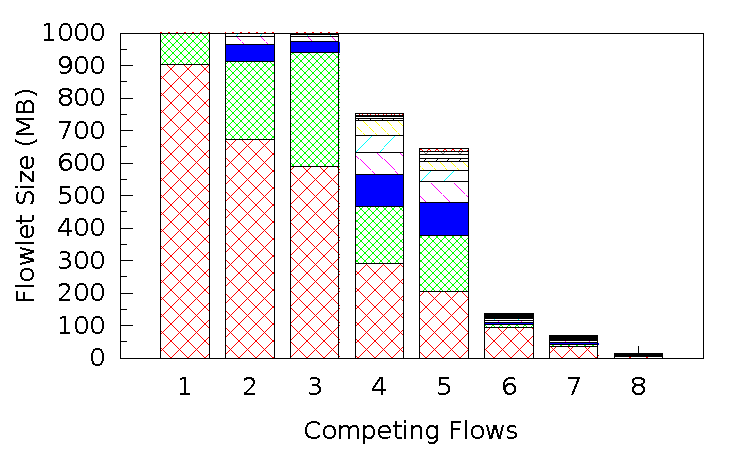
\includegraphics[width=0.7\textwidth]{presto/figures/flowlets/histo.pdf}
        \caption{Stacked histogram of flowlet sizes (in MB) for a 1 GB {\tt scp} file transfer. We vary the number of {\tt nuttcp}~\cite{nuttcp} background flows and
                denote them as {\em Competing Flows}. The size of each flowlet is shown within each bar, and flowlets
                are created whenever there is a 500 $\mu$s delay between segments. The top 10 flowlet sizes are shown here.
                We also analyzed the results of a 1 GB {\tt nuttcp}, {\tt ftp}, and a simple custom client/server transfer and found them
                to be similar. }
        \label{micro_flowlet_size}
\end{figure}

%\aditya{the following two paras don't flow well. they don't make a clear case for why flowlets is a bad idea and TSO segment level switching is a good idea. if reordering is the 100us flowlets' big problem then why not use our receiver-side reordering tricks with 100us flowlets? also it is not clear how were are overcoming reordering simply by relying on TSO segment switching}

%\eric{Rough estimates from our experiments with 100$\mu$s: ~90\% of flowlet sizes are 114KB or less with flowlets. ~00.1\% of flowlets are
%larger than 1 MB, with the largest ranging from 2.1-20.5MB. Some thoughts: (i) 100 $\mu$s flowlets can still have flowlet sizes larger 
%than switch buffers, which can cause congestion/loss when collision occur, (ii) given that flowlet with 100 $\mu$s does not prevent reordering,
%then why should we use flowlets at all? (iii) flowlets were really meant to have inactivity timers larger than the max difference in latency
%over any two paths, and buffer latency at one switch alone is ~4ms, so the use of flowlets on these small time scales is fundamentally
%flawed, (iv) flowlets are sensitive to traffic demand at sender, (v) flowlets are non-uniform in size, (vi) flowlets could break small 
%flows over multiple paths. Using TSO segment ensures: (i) small, uniform units of load-balancing, which means (ii) we are indenpendent
%of traffic demand, (iii) collisions are not a problem b/c TSO size is smaller than buffer size, (iv) most small flows are routed
%over the same path, (v) we do not impose too much computational overhead on sender/receiver and (vi) we still need to solve reordering.}

% Rough outline for next two paragraphs
% Problem with flowlets:
%  1. Sensitive to traffic patterns at the sender
%     a. In practice, we find this means the distribution of flowlet sizes is not uniform, and has a tail
%     b. These tails can still experience hash collisions, albeit less often.
%		i. congestion: lower throughput and to longer mice tail latencies
%  2. Needlessly break down small flows into several flowlets
%     a. Especially early in connection: 100us, 50 KB mice flows broken into 4-5 flowlets
%  3. Designed to be robust to reordering, but difficult to tune
%


Another possibility is to load balance on flowlets~\cite{conga,juniper-vcf}.  
A flow is comprised of a series of bursts, and a flowlet is created when
the inter-arrival time between two packets in a flow exceeds a threshold inactivity timer.  
In practice, inactivity timer values are between 100-500 $\mu$s~\cite{conga}. 
These values intend to strike a good balance between load balancing on a sub-flow level 
and acting as a buffer to limit reordering between flowlets.
Flowlets are derived from traffic patterns at the sender, and in practice this
means the distribution of flowlet sizes is not uniform. To analyze flowlet sizes, a simple experiment is shown in Figure~\ref{micro_flowlet_size}. 
We connect a sender and a receiver to a single switch and start an {\tt scp} transfer designed to 
emulate an elephant flow. Meanwhile, other senders are hooked up to the same switch and
send to the same receiver. We vary the number of these competing flows and show a stacked histogram of 
the top 10 flowlet sizes for a 1 GB {\tt scp} transfer with a 500 $\mu$s inactivity timer. 
The graph shows flowlet sizes can be quite large, with more than half the transfer being attributed
to a single flowlet for up to 3 competing flows. Using a smaller inactivity timer, such 100$\mu$s, helps (90\% of flowlet sizes are 114KB or less), but
does not prevent a long tail: 0.1\% of flowlets are larger than 1 MB, with the largest ranging from 2.1-20.5 MB.
Collisions on large flowlet sizes can lead to congestion.
The second problem with flowlets is that small inactivity thresholds, such as 100 $\mu$s, can lead to significant reordering.
Not only does this impact TCP performance (profiled in Section~\ref{sec:micro}), but it also needlessly 
breaks small flows into several flowlets. With only one flow in the network, we found a 50 KB
mice flow was broken into 4-5 flowlets on average. Small flows typically do not need to be
load balanced on a sub-flow level and need not be exposed to reordering.


%Another possibility is to load balance on flowlets~\cite{conga,juniper-vcf}.  A flow is typically comprised of a series of bursts, and each burst is defined as a flowlet. By monitoring the inter-arrival time of packets in a flow, one can easily define an inactivity timer to seperate flowlets.  In practice, intactivity timer values are between 100-500 $\mu$s~\cite{conga}. These values are intended to strike a good balance between creating enough opportunities to load balance on a sub-flow level and also ensure the reordering is limited at the destination due to the time buffer naturally incurred between flowlets.  We find, however, that it is difficult to strike a balance between achieving fine-grained, near-optimal load balancing and robustness against reordering. We perform a simple experiment in Figure~\ref{micro_flowlet_size}.  We connect a sender and a receiver to a single switch and start a transfer over an application designed to emulate an elephant flow ({\tt scp}). Meanwhile, we also hook up other senders to the same switch and have them send to the same reciever. We vary the number of competing flows and show a stacked histogram of the top 10 flowlet sizes for a 1 GB scp transfer with a 500 $\mu$s inactivity timer. \eric{Competing flows use nuttcp.} The graph shows flowlet sizes can be large, which means hash collisions can still occur on large flowlets.  Using a smaller timeout, such as 100 $\mu$s, creates smaller flowlets, but as we show in Section XXX, suffers from severe reordering that greatly reduces throughput and hurts applications.  \eric{mention creates congestion, which leads to lower thorughput and increase mice FCT latency}

% What do we want in sub-flow load balancing?
%  A. Want to move toward idealized ECMP: uniform sub-flow load balancing without the tail
%  B. Units should be as small as possible for fine-grained load balancing, but
%       not so small to be inefficient (TSO) or break small flows into parts
%  C. Independent of traffic patterns on sender
%  As a result, we settle on...

The shortcomings of the previous approaches lead us to reconsider on what granularity
load balancing should occur. 
%We take motivation from a best-case ECMP scenario. 
Ideally, sub-flow load balancing should be done on near uniform sizes.
%independent of traffic patterns on the sender to avoid long tails. 
Also, the unit of load balancing should be small to
allow for fine-grained load balancing, but not so small as to break small flows into 
many pieces or as to be a significant computational burden. As a result, we
propose load balancing on 64 KB units of data we call {\em flowcells}. Flowcells
have a number of advantages. First, the maximum segment size supported by TSO
is 64 KB, so flowcells provide a natural interface to high speed optimizations provided
by the NIC and OS and can scale to fast networking speeds. Second, an overwhelming fraction of mice flows are less than 64 KB in size
 and thus do not have to worry about reordering~\cite{benson10,vl2,kandula2009nature}.
Last, since most bytes in datacenter networks originate from elephant flows~\cite{kandula2009nature,benson10,dctcp},
this ensures that a significant portion of datacenter traffic is routed on uniform
sizes. While promising, this approach must combat reordering to be effective. 
Essentially we make a trade-off: 
%we provide line rate load balancing in the most effective
%manner as to avoid congestion and then handle reordering head-on at the receiver.
the sender avoids congestion by providing fine-grained, near-uniform load balancing,
and the receiver handles reordering to maintain line-rate.


%We highlight the challenges of this approach
%in the next subsection and provide a design to mitigate reordering problems in Section~\ref{sec:design}.

%In order to obtain fine-grained, near-optimal load balancing, we should stripe on a granularity
%that is indendpent of traffic patterns, near-uniform in size, and as small as possible while still
%scaling to fast network speeds.
%Therefore, we argue the TSO segment~\keqiang{what about saying maximum TSO segment size (64KB), each TSO segment's size is bounded by maximum TSO size} 
%is the natural granularity in which to load balance. Doing so
%provides several benefits. First, TSO segments are small and near-uniform in size, so an
%effective load-balancing scheme should be able to closely track the optimal case of per-packet
%load balancing, but without the additional computational overhead.
%Second, the TSO engine in the NIC will ensure that all packets created from a TSO segment will contain the same
%header information. We show in Section XXX how this is important to deal with reordering because
%we can easily impart metadata on all packets within a segment that help us distinguish loss from 
%ordering~\keqiang{all the packets within the same flowcell contain the same flowcell id.  
%"all packets created from a TSO segment will contain the same
%header information" is fine but a flowcell can contrain several TSO segments depending on TSO segment size}.
%Last, small flows less than 64 KB in size will actually be routed over the
%same path in the network, meaning a very large fraction of mice flows will not be routed on a subflow
%level and thus do not have to worry about reordering~\cite{benson10,vl2,kandula2009nature}~\keqiang{Around 90\% of datacenter flows' sizes are smaller than 64KB~\cite{benson10}, 
%meaning the overwhelming majority is load balanced like ECMP and we only need to engineering the left 10\%}.
%\eric{need to mention that we can combine segments as long as not above 64 KB, so not really
%per TSO segment. helps in small flows.}
%While promising, this approach has a major challenge: reordering. We highlight these challenges
%in the next subsection and provide a design to mitigate the problems in Section~\ref{sec:design}.

\tightparagraph{Per-Hop vs End-to-End Multipathing}
The last design consideration is whether multipathing should be done on a local, per-hop level (\eg{}ECMP), or
on a global, end-to-end level. In Presto, we choose the latter: pre-configured end-to-end paths
are allocated in the network and path selection (and thus multipathing) is realized by having the network edge
place flowcells onto these paths. 
Presto can be used to load-balance in an ECMP style per-hop manner, but the choice of end-to-end 
multipathing provides additional benefits due to greater control of how flowcells are mapped to
paths. Per-hop multipathing can be inefficient
under asymmetric topologies~\cite{wcmp}, and load-balancing on a global end-to-end level can allow
for weighted scheduling at the vSwitch to rebalance traffic. This is especially important when failure occurs.
The second benefit is flowcells can be assigned over multiple paths very evenly
by iterating over paths in a round-robin, rather than randomized, fashion. 

%As we show
%in Section~\ref{sec:micro}, randomization in per-hop multipathing can lead to "unluckiness" where
%multiple flowcells get sent to the same link over a small timescale by multiple flows. This transient congestion
%can lead to increased buffer occupancy and higher delays in the network. These benefits can
%fundamentally be provided at the per-hop level (\cite{wcmp} handles asymmetry), but require changes to networking firmware. 
%These considerations motivate us to utilize end-to-end multipathing, but Presto can also
%use per-hop multipathing when conveinent.

\subsection{Reordering Challenges}
%The above design decisions in Presto cause following main challenges:
Due to the impact of fine-grained, flowcell-based load balancing, Presto must account for reordering. Here, we 
highlight reordering challenges. The next section shows how Presto deals with these concerns.

%\tightparagraph{Soft Edge Distributed Load Balancing}
%There are two main challenges in implementing load balancing at the soft edge. First, the implementation
%must scale to fast networking speeds because networking at 10+ Gbps can have significant overhead if not carefully
%considered. Therefore, in order to achieve line rate, great care must be taken to ensure that load balancing
%schemes are light-weight, simple and can take advantage of optimizations provided by the NIC and OS.  
%The second major problem is how to load balance in a distributed fashion at the vSwitches in such
%a way that the load balancing performs well globally.
%Nodes must ensure they are spreading
%their traffic equally throughout the network, but in a low-overhead fashion that does not require detailed
%topographical information about the network, real-time traffic matrices, or strict coordination
%with other senders.

%\eric{several things to add: in presto, we can just make dumb edge decisions and not have to worry
%about (i) the traffic patterns, that is who else is sending, (ii) topology asymmetry. Basically,
%we want to highight that the vSwitch shouldn't require a lot of detailed network-wide information,
%but should be able to somehow still load balance in a way that performs very well globally.}

\tightparagraph{Reordering's Impact on TCP} The impact of reordering on TCP is well-studied~\cite{leung2007overview,paxson1997end}. 
Duplicate acknowledgments caused by reordering
can cause TCP to move to a more conservative sender state and reduce the sender's congestion window.
Relying on parameter tuning, such as adjusting the DUP-ACK threshold, is not ideal because 
increasing the DUP-ACK threshold increases the time to recover from real loss. Other TCP settings
such as Forward Acknowledgement (FACK) assume un-acked bytes in the SACK are lost and degrade
performance under reordering. 
A scheme that introduces reordering should not rely on careful configuration of TCP parameters
because (i) it is hard to find a single set of parameters that work effectively over multiple 
scenarios and (ii) datacenter tenants should not be forced to constantly tune their networking stacks.
Finally, many reordering-robust variants of TCP have been proposed~\cite{rr-tcp,blanton2002making,tcp-pr}, but
as we will show, GRO becomes ineffective under reordering. Therefore, reordering should
be handled below the transport layer.

\tightparagraph{Computational Bottleneck of Reordering}
Akin to TSO, Generic Receive Offload (GRO) mitigates the computational burden of receiving
1500 byte packets at 10 Gbps. GRO is implemented in the kernel of the hypervisor,
and its handler is called directly by the NIC driver. It is responsible
for aggregating packets into larger segments that are pushed up to OVS and the TCP/IP stack. 
GRO is implemented in the Linux kernel and is used even without virtualization. Similar
functionality can be found in Windows (RSC~\cite{ms-rsc}) and hardware (LRO~\cite{grossman2005large}).

Because modern CPUs use aggressive prefetching, the cost of receiving
TCP data is now dominated by per-packet, rather than per-byte, operations.
As shown by Menon~\cite{optimize-tcp-receive},  the majority of this overhead comes from
buffer management and other routines not related to protocol processing, and therefore 
significant computational overhead can be avoided by aggregating "raw" packets from
the NIC into a single {\tt sk\_buff}.
%\footnote{Refer to~\cite{linuxgro,optimize-tcp-receive} for detailed study and explanation}
Essentially, spending a few cycles to aggregate packets within GRO creates less segments for
TCP and prevents having to use substantially more cycles at higher layers in the networking stack.
Refer to~\cite{linuxgro,optimize-tcp-receive} for detailed study and explanation.

To better understand the problems reordering causes, a brief description of  
the TCP receive chain in Linux follows. First, interrupt coalescing allows the NIC to create an interrupt for a batch of packets~\cite{mogul1997eliminating,understanding-linux-network},
which prompts the driver to poll the packets into an aggregation queue. Next, the driver
invokes the GRO handler, located in the kernel, which
{\em merges} the packets into larger segments. The merging continues,
possibly across many polling events, until a segment
reaches a threshold size, a certain age, or cannot be combined with the incoming packet. Then, the
combined, larger segment is {\em pushed up} to the rest of the TCP/IP networking stack. The GRO process is
done on a per-flow level. With GRO disabled, throughput drops to around
5.7-7.1 Gbps and CPU utilization spikes to 100\% (Section~\ref{sec:micro} and~\cite{bullettrains}). 
Receive offload algorithms, whether in hardware (LRO)~\cite{grossman2005large,open-lro} or in software (GRO), are usually
{\em stateless} to make them fast: no state is kept beyond the segment being merged.


%\begin{figure}[!htb]
%        \centering
%  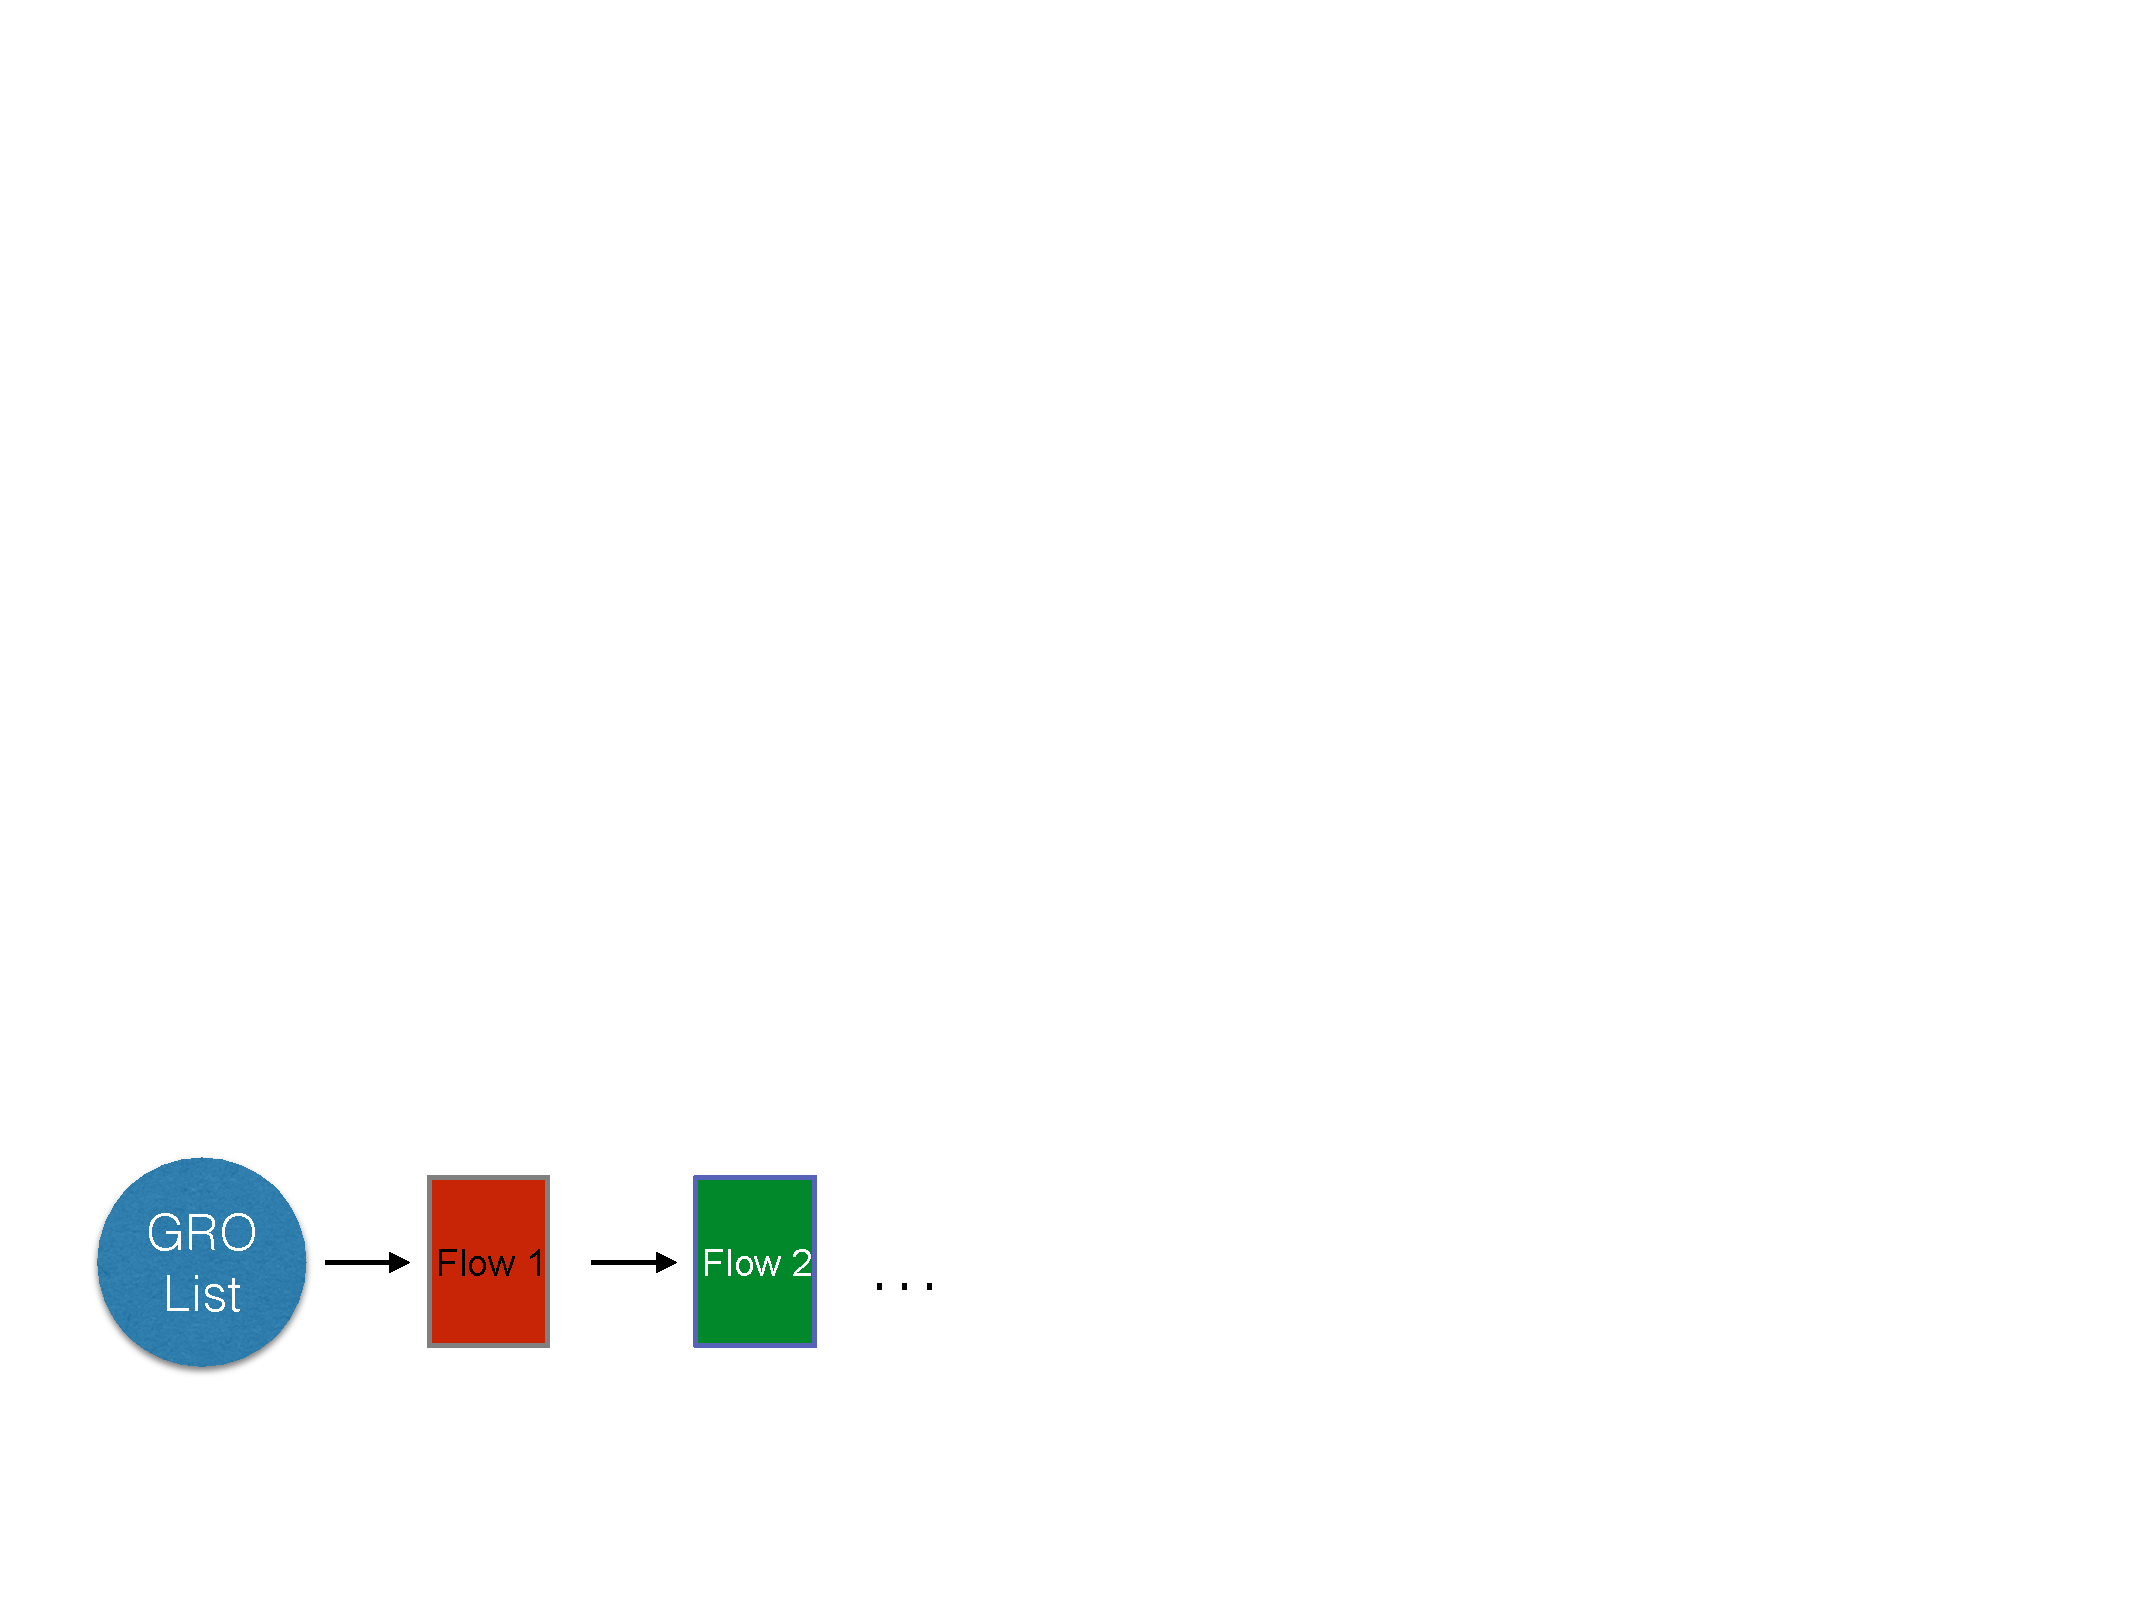
\includegraphics[width=0.45\textwidth]{presto/figures/gro-design/gro.pdf}
%        \caption{GRO design. FIX ME!}
%        \label{gro-design}
%\end{figure}

\begin{figure}[!t]
        \centering
  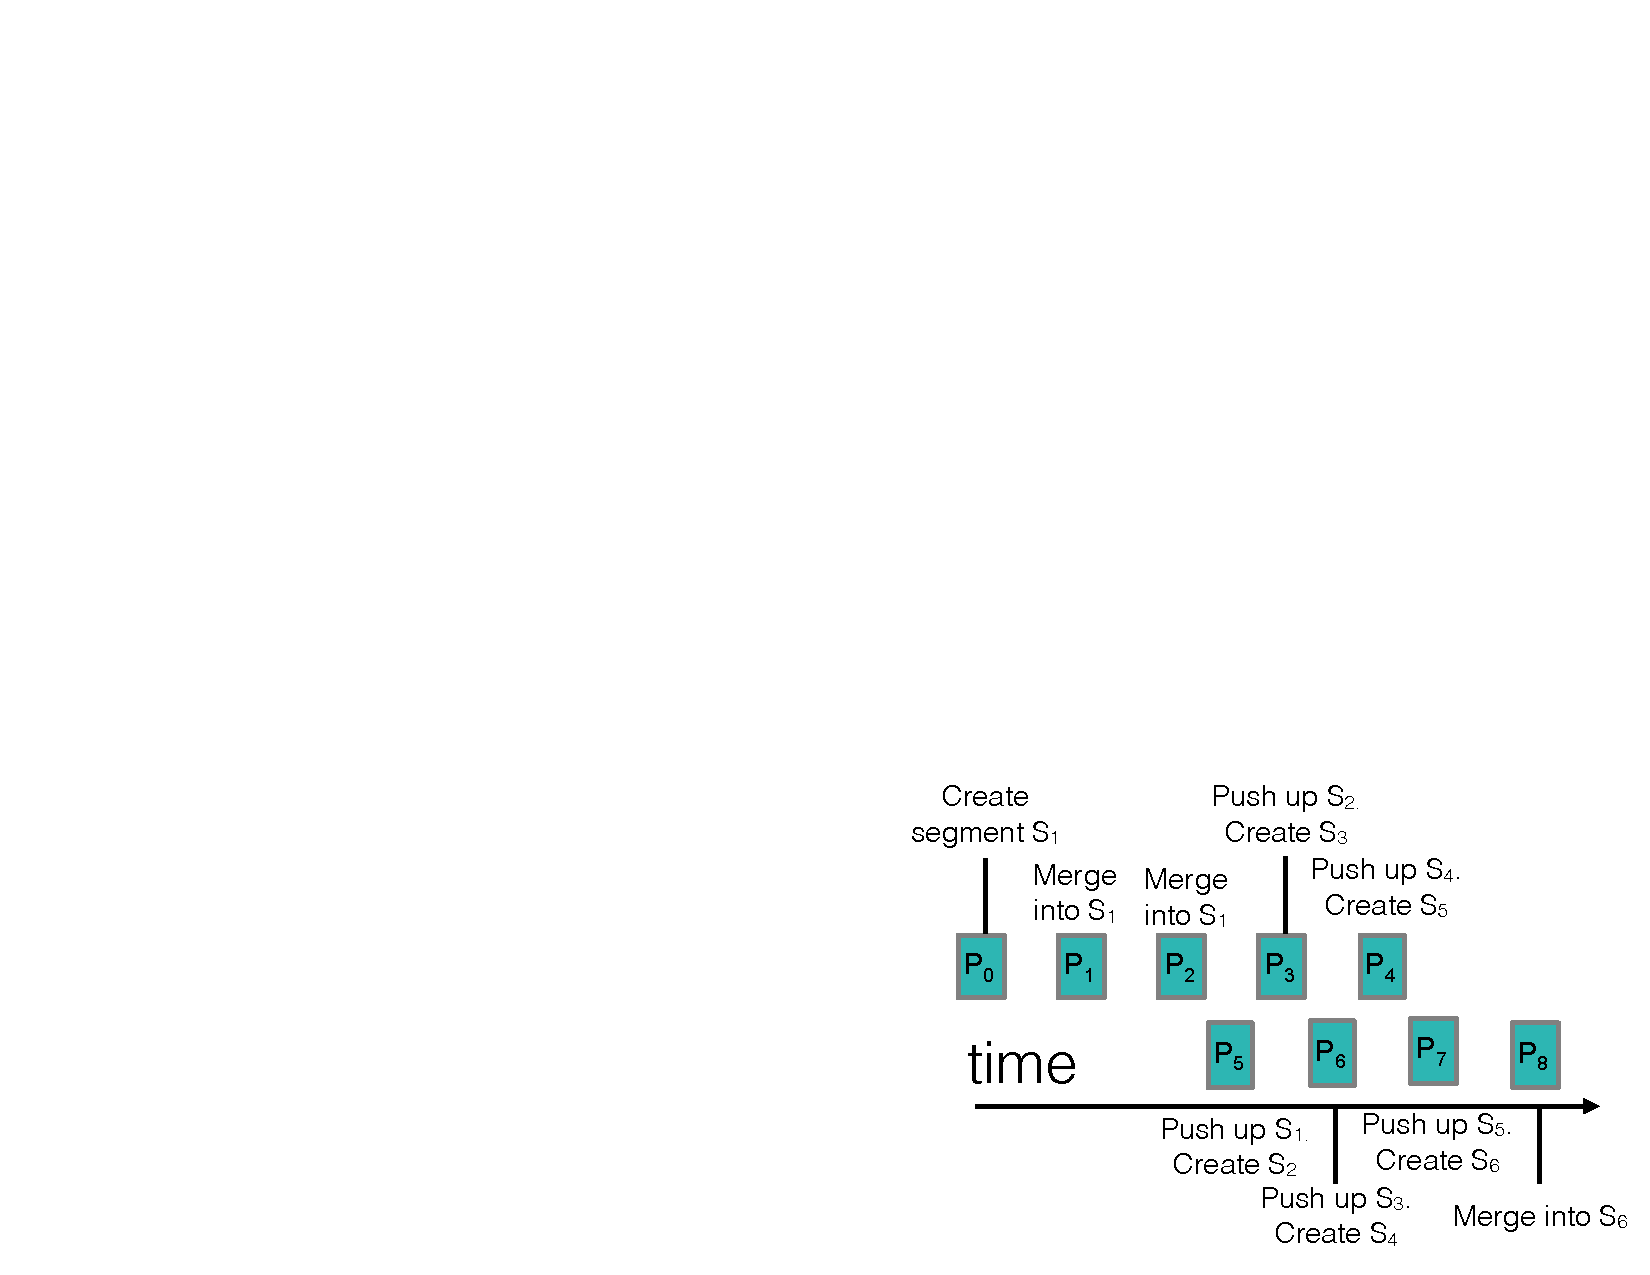
\includegraphics[width=0.7\textwidth]{presto/figures/gro-design/gro-break.pdf}
        \caption{GRO pushes up small segments ($S_i$) during reordering.}
        \label{gro-break}
\end{figure}


We now uncover how GRO breaks down in the face of reordering. Figure~\ref{gro-break} shows the impact of reordering on GRO.  Reordering does not allow the segment to grow: each reordered packet cannot be merged with the existing segment, and thus the previously created segment must be pushed up. With extreme reordering, GRO is effectively disabled because small MTU-sized segments are constantly pushed up. This causes (i) severe computational overhead and (ii) TCP to be exposed to significant amounts of reordering. We term this the {\em small segment flooding} problem.

Determining where to combat the reordering problem has not previously taken the small segment flooding problem into account.  Using a reordering buffer to deal with reordered packets is a common solution (\eg{}works like~\cite{drb} re-sort out-of-order packets in a shim layer below TCP), but a buffer implemented above GRO cannot prevent small segment flooding.  Implementing a buffer below GRO means that the NIC must be changed, which is (i) expensive and cumbersome to update and (ii) unlikely to help combat reordering over multiple interrupts.

In our system, the buffer is implemented in the GRO layer itself.  We argue this is a natural location because GRO can
directly control segment sizes while simultaneously limiting the impact of reordering. 
Furthermore, GRO can still be applied on packets pushed up from LRO, which means hardware doesn't have to be modified
or made complex.
Implementing a better GRO algorithm has multiple challenges. The algorithm should be light-weight to scale to fast networking speeds. Furthermore, an ideal scheme should be able to distinguish loss from reordering.  When a gap in sequence numbers is detected (\eg{}when $P_5$ is received after $P_2$ in Figure~\ref{gro-break}), it is not obvious if this gap is caused from loss or reordering.  If the gap is due to reordering, GRO should not push segments up in order to try to wait to receive the missing gap and merge the missing packets into a preestablished segment.  If the gap is due to loss, however, then GRO should immediately push up the segments to allow TCP to react to the loss as fast as possible. Ideally, an updated GRO algorithm should ensure TCP does not perform any worse than a scheme with no reordering. Finally, the scheme should adapt to prevailing network conditions, traffic patterns and application demands.




%\include{vnd/vnd}
%\include{perfsight/perfsight}
%
{\bf Load Balancing in Datacenters} 
%Load balancing in datacenter networks has been the focus of several studies.
MPTCP~\cite{mptcp,dc-mptcp} is a transport protocol that uses subflows to 
transmit over multiple paths.
CONGA~\cite{conga} and Juniper VCF~\cite{juniper-vcf} both employ congestion-aware flowlet switching~\cite{flowlet} on
specialized switch chipsets to load balance the network.
RPS~\cite{packetspray} and DRB~\cite{drb} evaluate per-packet load balancing on symmetric 1 Gbps networks
at the switch and end-host, respectively.
The CPU load and feasibility of end-host-based per-packet load balancing for 10+ Gbps networks remains open.
%Per-packet load balancing can incur significant end-host overhead for DRB
%if not resorting to jumbo frames.
%Packet reordering problem is not well considered in both RPS and DRB.
%RPS and DRB may perform worse than ECMP in case of topology asymmetry.
Hedera~\cite{hedera}, MicroTE~\cite{microte} and Planck~\cite{planck} use centralized traffic engineering to
reroute traffic based on network conditions.
FlowBender~\cite{flowbender} reroutes flows when congestion is detected by end-hosts and 
Fastpass~\cite{fastpass} employs a centralized arbiter to schedule path selection for each packet.
As compared to these schemes, Presto is the only one that proactively load-balances at line rate for fast networks
in a near uniform fashion without requiring additional infrastructure or changes
to network hardware or transport layers. Furthermore, to the best of our knowledge, Presto is
the first work to explore the interactions of fine-grained load balancing with built-in
segment offload capabilities used in fast networks.
%\textcolor{blue}{~\cite{eden} also advocates to implement network functions such as load balancing 
%at datacenter end hosts.}

{\bf Reducing Tail Latency}
%Detail~\cite{detail} summarizes the causes of long tails of flow completion time---
%1)packet loss and retransmissions,
%2)absence of flow prioritization and 3)uneven load balancing.
%Reducing tail latencies of small mice flows has also been actively studied.
DeTail~\cite{detail} is a cross-layer network stack designed to reduce the tail of flow completion times.
%link layer uses port buffer occupancy to construct lossless fabric,
%network layer performs per-packet adaptive load balancing based on port buffer occupancy,
%transport layer relies upon congestion notifications
%derived from port buffer occupancies,
%finally Detail lets application layer specify flow priorities to
%avoid head-of-line blocking of elephant flows for mice time-sensitive flows.
%Detail modified many layers (including the switch) and is hard to deploy using
%current hardware and network stack.
DCTCP~\cite{dctcp} is a transport protocol that uses the portion of marked packets 
by ECN to adaptively adjust sender's TCP's congestion window to reduce switch buffer occupancy.
%Thus, DCTCP can reduce switch buffer occupancy and reduce flow completion time.
HULL~\cite{hull} uses Phantom Queues and congestion notifications to cap link utilization and prevent congestion.
%HULL uses packet pacing to combat with traffic burstiness in order to leave "bandwidth headroom".
In contrast, Presto is a load balancing system that naturally improves 
the tail latencies of mice flows by uniformly spreading traffic in 
fine-grained units.
%We share the overall goal of reducing mice tail latencies, but instead explore how
%fine-grained load balancing can provide a solution.
QJUMP~\cite{qjump} utilizes priority levels to 
allow latency-sensitive flows to "jump-the-queue" over low priority flows.
PIAS~\cite{bai2015information} uses priority queues to mimic the Shortest Job First principle to reduce FCTs.
%solve the network interference problem caused by elephant and mice flows 
%for datacenter networks. High priority packets are rate-limited 
%at the end-host and can "jump-the-queue" over packets with 
%lower priorities. PIAS~\cite{pias} mimics the Shortest Job First (SJF) 
%principle to reduce flow completion times. It gradually decreases 
%the priority level assigned to a flow based on its flow size.
%Presto is complementary and could be applied on each priority level.
%DIBS~\cite{dibs} detours packets of a congested switch port to a randomly 
%picking neighboring switch to reduce packet drops.
Last, a blog post by Casado and Pettit~\cite{vmware} summarized
four potential ways to deal with elephants and mice, with one advocating
to turn elephants into mice at the edge. 
We share the same motivation and high-level
idea and design
a complete system that addresses many practical challenges of using
such an approach.


{\bf Handling Packet Reordering}
%Many schemes have tried to mitigate the impact of reordering.
TCP performs poorly in the face of reordering, and thus several studies
design a more robust alternative~\cite{rr-tcp,blanton2002making,tcp-pr}.
Presto takes the position that reordering should be handled below TCP in the existing 
receive offload logic.
In the lower portion of the networking stack, SRPIC~\cite{wu2009sorting} sorts reordered packets 
in the driver after each interrupt coalescing event. While this approach can help
mitigate the impact of reordering, it does not sort packets across interrupts, have a 
direct impact on segment sizes, or distinguish between loss and reordering. 
%SRPIC is 
%complementary to our approach because their actions are taken in the driver, before packets
%are pushed to GRO.
%RR-TCP~\cite{rr-tcp} proposed to extend TCP sender to detect and recover from false fast retransmits using DSACK information. 
%As we show, fixing TCP itself cannot solve all the problems incurred by packet reordering.
%\eric{i have some LRO references in the patent slides that we need to make sure are cited somewhere} 
%Instead, Presto's chunking scheme leverages the fact that all the packets going through the same path are in order and has two nice properties:
%1)Presto uses chunkid to make the task of distinguishing packet loss from temporary packet reordering much simpler. 
%2)Presto only needs to make sure the chunks are in order instead of packets, thus reducing per-packet processing overhead.

{\bf Congestion control for DCNs}
%\crs{Rather than proposing a new congestion control algorithm, our work investigates if congestion control can be moved to the vSwitch.
%Thus, many of the following schemes are complimentary.}
DCTCP~\cite{dctcp} is a seminal TCP variant for datacenter networks.
Judd~\cite{judd2015nsdi} proposed simple yet practical fixes to enable DCTCP in production networks.
TCP-Bolt~\cite{stephens2014practical} is a variant of DCTCP for PFC-enabled lossless Ethernet.
%DCQCN~\cite{zhu2015congestion} is a rate-based congestion control scheme implemented in NICs
%for QCN-based~\cite{qcn} RDMA deployments.
DCQCN~\cite{zhu2015congestion} is a rate-based congestion control scheme (built on DCTCP and QCN) to
support RDMA deployments in PFC-enabled lossless networks.
TIMELY~\cite{mittal2015timely} and DX~\cite{lee2015accurate}
use accurate network latency as the signal to perform congestion control.
TCP ex Machina~\cite{winstein2013tcp} uses computer-generated congestion control rules.
PERC~\cite{jose2015high} proposes proactive congestion control to improve convergence.
ICTCP's~\cite{wu2010ictcp} receiver monitors incoming TCP flows and
modifies~\rwnd{} to mitigate the impact of incast, but this cannot
provide generalized congestion control like~\acdc{}.
Finally, efforts~\cite{dell-toe,chelsio-toe} to
implement TCP Offload Engine (TOE) in specialized NICs are not widely deployed for reasons noted in~\cite{mogul2003tcp,linux-toe}.
vCC~\cite{vcc} is a concurrently designed system that shares~\acdc{}'s goals and some of its design details.
The paper is complementary in that some items not addressed in~\acdc{} are presented, such as a more detailed
analysis of the ECN-coexistence problem, an exploration of the design space, and a theoretical proof of
virtualized congestion control's correctness.~\acdc{} provides an in-depth design and thorough evaluation of
a DCTCP-based virtualized congestion control algorithm on a 10 Gbps testbed.


{\bf Bandwidth allocation} Many bandwidth allocation schemes have been proposed.
Gatekeeper~\cite{rodrigues2011gatekeeper} and EyeQ~\cite{jeyakumar2013eyeq} abstract the network as a single
switch and provide bandwidth guarantees by managing each server's access link.
Oktopus~\cite{Ballani2011oktopus} provides fixed performance guarantees within virtual clusters.
SecondNet~\cite{Guo2010Secondnet} enables virtual datacenters with static bandwidth guarantees.
Proteus~\cite{Xie2012Proteus} allocates bandwidth for applications with dynamic demands.
Seawall~\cite{shieh2011sharing} provides bandwidth proportional to a defined weight by
forcing traffic through congestion-based edge-to-edge tunnels.
NetShare~\cite{Lam2012NetShare} utilizes hierarchical weighted max-min fair sharing to tune relative bandwidth allocation for services.
FairCloud~\cite{Popa2012Faircloud} identifies trade-offs in minimum
guarantees, proportionality and high utilization, and designs schemes over this space.
Silo~\cite{jang2015silo} provides guaranteed bandwidth, delay and burst allowances through a novel VM placement and admission
algorithm, coupled with a fine-grained packet pacer. 
~\acdc{} is largely complimentary to these schemes because it is a transport-level solution.

{\bf Rate limiters}
SENIC~\cite{niranjan2013fastrak}
identifies the limitations of NIC hardware rate limiters (\ie{}, not scalable) and
software rate limiters (\ie{}, high CPU overhead) and uses the CPU to enqueue packets
in host memory and the NIC. Silo's pacer injects void packets into
an original packet sequence to achieve pacing. FasTrack~\cite{niranjan2013fastrak} offloads
functionality from the server into the switch for certain flows.
%~\acdc{} prevents
%TCP flows from sending in the first place and can be used in conjunction with these
%schemes.


%\chapter{Conclusion}
\label{chap:conc}
In this thesis, we have demonstrated new network problems in the cloud environment
and our approaches to solve them. We have shown the feasibility and performance
of our approach. 
Here, we highlight the main contributions of our works, and then close this thesis with
a discussion of options for future work.
\section{Contributions}
\paragraph{VND.} We proposed a virtual network diagnostic service from the cloud provider
to its cloud tenants.
%  makes a case for providing virtual network diagnosis as a service in the cloud.  
We identified a set of technical challenges in providing such a service and propose
a Virtual Network Diagnosis (VND) service framework.  VND exposes abstract
configuration and query interfaces for cloud tenants to troubleshoot
their own virtual networks. It controls software switches to collect
flow traces, distributes traces storage, and executes distributed
queries for different tenants for network diagnosis. It reduces the
data collection and processing overheads by performing local flow
capture and on-demand query execution. 
  %Our evaluation shows the feasibility of providing a virtual network diagnosis service in the cloud. VND is prompt to respond tenant's diagnosis request and introduces acceptable overhead.
Our experiments validated the functionality of VND approach and showed its feasibility 
in terms of quick service response and acceptable overhead; our simulation
proved the VND architecture cloud be scaled to the size of a real data center network.
\paragraph{\Name.}
The new ``software data
planes'' in the cloud infrastructure are susceptible to at least three new classes of
performance problems. To diagnose such problems, we designed,
implemented and evaluated \Name, a ground-up system that works by
extracting comprehensive low-level information regarding packet
processing and I/O performance of the various elements in the
software data plane. \Name then analyzes the information gathered in
various dimensions (e.g., across all VMs on a machine, or all VMs
deployed by a tenant). By looking across aggregates, we showed that it
becomes possible to detect and diagnose key performance
problems. Our experimental results showed that our framework can result in
accurate detection of the root causes of key performance problems in
software data planes, and it imposes very little overhead.
\section{Future Work}
Our study has not covered all aspects of the cloud infrastructure. There
are still other network troubleshooting issues in the cloud infrastructure,
which we consider as research areas for future work. In addition, our study of the 
network problems also points out a way to improve the network performance.

\paragraph{Control Plane.} The cloud control plane translates
and deploys management policies (e.g., virtual networks) into low-level devices. There are several
layers in this process: the management policy, the logic view, the physical view, and the device
states. Diagnostic tools for traditional networks usually target the physical-view layer and the
device states; they have proposed network-wide invariants such as loop-free, reachability in these
two layers. I argue that in the public cloud, more invariants need to be guaranteed, such as isolation
and fault tolerance. I intend to model this layer-by-layer translation and the invariants. In addition,
I believe we need to use the actual data plane behaviors to verify the network invariants instead of the
states in the control plane (as is done in current solutions); 
to implement this, we can make use of existing techniques such as sFlow,
NetFlow or VND to capture the network traffic and to verify whether the data plane behavior violates
the network invariants.

\paragraph{Software Data Plane Optimization.} An observation of our data plane diagnostic work 
is that processing overheads is imposed in the software data plane, causing unsatisfactory
performance (e.g., low throughput). The overhead is usually
caused by uncoordinated design of data plane components (these components are usually designed
for generic usage). In a specific environment (e.g., multi-tenant cloud), the software data plane can
be further optimized. For example, two VMs in the same physical server can exchange network
traffic with zero memory copy; VM outgoing traffic can bypass the NAPI routine to the NIC directly.
I intend to further optimize the the software data plane in the context of multi-tenant clouds.

I would like to discover whether the software data plane can be software-defined.
The optimization examples mentioned above actually design new ``short-cut" datapaths for
network traffic to accelerate processing speed. It is possible to control the datapath in the software
data plane, so that different flows go through different datapaths and achieve different benefits.
For example, trusted VMs can exchanges packets directly without going through virtual switches,
while untrusted VMs should not for security reasons; 
delay-sensitive middlebox traffic can output directly to
the physical NIC, while others are put into the CPU backlog queue for bulk processing. This requires
a new design and implementation of the software data plane and the comprehensive evaluation of different practices.

%\cite{example}


\bibliography{refs}              % Make the bibliography
\bibliographystyle{plain}

%\begin{appendices}               % Start of the Appendix Chapters.  If there is only
                                 % one Appendix Chapter, then use \begin{appendix}
%\include{code}                   % Including computer code listings
%\include{bibref}                 % a BibTeX reference
%\include{math}                   % Complex Equations from the UW Math Department
%\include{acro}                   % A discussion on generating PDF files.
%\end{appendices}                 % End of the Appendix Chapters.  ibid on \end{appendix}
%\include{vita}                  % Optional Vita, use \begin{vita} vita text \end{vita}
\end{document}
